\documentclass[11pt, oneside]{article}   
\usepackage{geometry}              	
\usepackage{adjustbox}
\usepackage{pdfpages}  	
\usepackage[nottoc]{tocbibind}
\usepackage{graphicx}
\usepackage{caption}						
\usepackage{amssymb}
\usepackage{booktabs} % To thicken table lines
\usepackage{amsmath}
\usepackage{pdfpages} 
\usepackage{longtable}
\usepackage{subfig}
\usepackage{url}
\usepackage{hyperref}
\hypersetup{colorlinks,linkcolor={blue},citecolor={blue},urlcolor={red}}  
\usepackage{titlesec}
\usepackage[english]{babel}
\usepackage[utf8]{inputenc}
\usepackage[font=small,labelfont=bf]{caption}

\title{EOSC 595: Directed study, Arctic Climate change - A review on the usage of ERA5 reanalysis in the Arctic region  }
\nonstopmode
%\usepackage[utf-8]{inputenc}
\usepackage{graphicx} % Required for including pictures
\usepackage[figurename=Figure]{caption}
\usepackage{float}    % For tables and other floats
\usepackage{verbatim} % For comments and other
\usepackage{amsmath}  % For math
\usepackage{amssymb}  % For more math
\usepackage{fullpage} % Set margins and place page numbers at bottom center
\usepackage{paralist} % paragraph spacing
\usepackage{listings} % For source code
\usepackage{subfig}   % For subfigures
%\usepackage{physics}  % for simplified dv, and 
\usepackage{enumitem} % useful for itemization
\usepackage{siunitx}  % standardization of si units
% \usepackage{amsmath}
\usepackage{mathtools}% Loads amsmath

\usepackage{tikz,bm} % Useful for drawing plots
%\usepackage{tikz-3dplot}

\usepackage{enumitem}
%\renewcommand{\theenumi}{\Alph{enumi}}


\usepackage{csquotes}



%\renewcommand{\labelenumii}{\Arabic{enumii}}


\begin{document}

\begin{center}
	\hrule
	\vspace{.4cm}
	{\textbf { \large EOSC 595: Directed study, Arctic Climate change \\ A review on the usage of ERA5 reanalysis in the Arctic region}}
\end{center}
{\textbf{Name:}\ Ruth Moore \hspace{\fill} }\textbf{Date:} March 3rd 2022   \\
	\hrule


\hfill
\hfill
 \hfill
\hfill

\section{Introduction}

{\color{blue}look at different papers which have reviewed ERA for use in other regions and base my paper off of it}


Due to temporal and spatial biases, complete weather measurements for the past are not always available. Historical measurements which are available are not evenly distributed around the globe, particularly for areas in harsh environments with small populations, such as the Arctic region.

Reanalysis data sets combine weather measurements from the past with up to date climate and weather models to form a complete picture of weather patterns in the past. These data sets provide comprehensive weather and climate conditions at regular intervals overtime and are used in atmospheric dynamics, climate stability and for evaluating climate models. In many study in the Arctic region, reanalysis output are used in replacement of historical measurements since historical record is sparce.

ERA5 is often used as a data product when comparing CMIP and other model outputs to 'observations', such as in \cite{ford2022arctic} where CMIP and ERA5 are compared to evaluate hydrological changes due to sea ice loss and in \cite{rantanen2022arctic} where the Arctic is seen to have warmed 4 times more than the global average. However, studies show that ERA5 overestimates both precipitation amount and frequency in the Arctic region (my work) {\color{blue} develop this point with more references}, and therefore should not blindly be used as a data product without thorough evaluation of its limitations and biases within the Arctic. 

Understanding of these limitations, particularly with precipitation is crucial for work in the Arctic and for global climate evaluation as a whole. To quote Boisvert in \cite{boisvert2018intercomparison}; "[precipitation] is one of the most poorly constrained variables in atmospheric reanalyses". 


A large section of this review paper will focus on precipitation, since precipitation is one of the most rapidly changing variables in the Arctic as we see a transition from snow to rain, and it is one of the most limited and difficult to use reanalysis products, as will be explained in section \ref{precipitation}.

This review will look at why we use reanalysis, will discuss the major atmospheric realanalysis products available in the Arctic, introducing ERA5 as the most relaible one. Then a discussion on major variable related to the atmospheric hydrological cycle is given, where precipitation and trace precipitation are discussed in depth. Finally a review on regional differences is given with a discussion on knowledge gaps. 


\section{Why we use reanalysis}
Reanalysis datasets ensure that we have a more thorough and robust dataset of meteorogical information for the globe. They are particularly useful for work in the Arctic since direct measurements are often limited due to temporal and spatial difficulties associated with remote regions.

Assimilated observations are observational records which are inputted directly into reanalysis models. In most reanalyses products, temperature is assmilated. 

The satelite era is defined as the period between 1979 to present day, which represents a more accurate output period of reanalysi datasets as it is the year when satellite observations began to be assimilated into reanalsysis products. 


Reanalysis products are not prefect and come with distinct limitations, particulary in the Arctic where assimliation is low due to limitations in observational records. Some of these limiations include a warm bias over sea ice when compared to buoy measurments \cite{wang2019comparison} and the presence of trace precipitation \cite{boisvert2018intercomparison}, this is discussed in detail in section \ref{traceprecip}.

Reanalysis models also often have biases due to changing observation methods. This aside, they are useful and critical to researching climate in the recent past. 

\section{Reanalysis products available in the Arctic}

When comparing different products use a figure which looks like this 

\begin{figure}[ht]
    \centering
    \vspace{-4mm}
    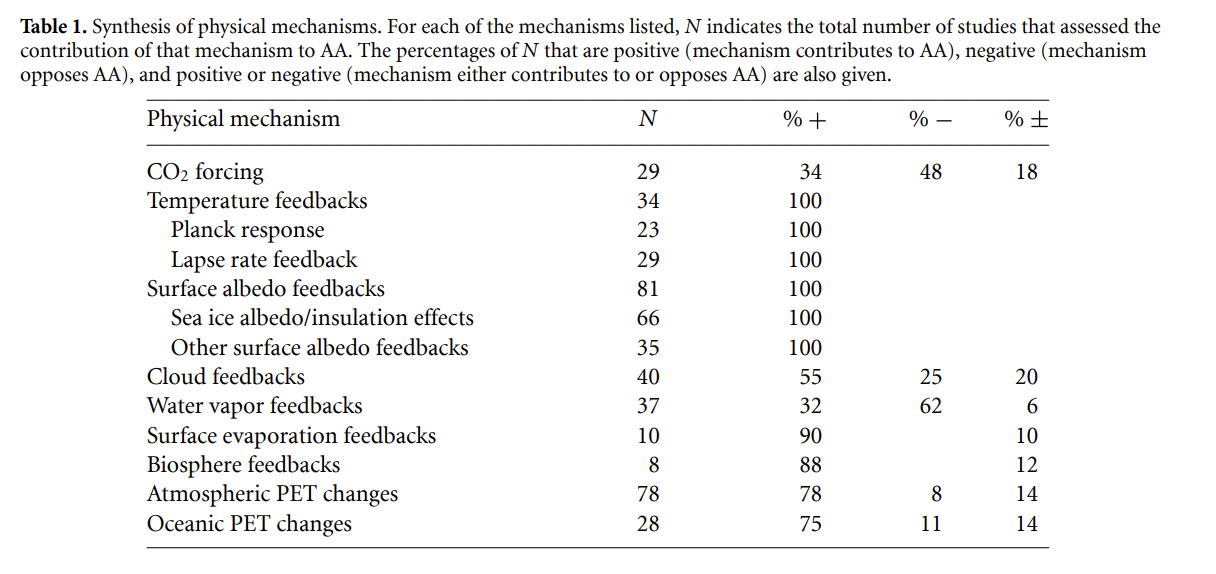
\includegraphics[width=80mm]{previdi_comparasion_mechanisms.png}
    \vspace{-4mm}
    \caption{from \cite{previdi2021arctic} }
    \label{f:previdi2021arctic}
\end{figure}
\section{An evaluation of ERA-5}
WHY IS ERA5 good?

How have other studies compared ERA5 and what have they said?

There are a number of different reanalysis datasets available for study in the Arctic. 


\section{An introduction to ERA5}
ERA5 is the fifth generation ECMWF (European Centre for Medium-Range Weather Forecasts) atmospheric reanalysis for the globe. The product spans from 1940 to present day and is available to download at \url{https://cds.climate.copernicus.eu/cdsapp#!/dataset/reanalysis-era5-single-levels?tab=overview}. ERA5 provides hourly measurements for a large number of atmospheric, land and oceanic variables \cite{hersbach2020era5}. 
ERA5 grid cells are 0.25° x 0.25°, which roughly corresponds to 31km x 31km, with atmospheric resolution to 80km over 137 levels. 2D and 3D data are available with daily and monthly estimates available in addition to hourly estimates. 

Terrestrial
2
higher


terrestrial

ERA-5 was chosen specifically for this review as it is the most reliable global reanlaysis for the Arctic right now. It highest correlation coefficients compared with experimental weather data, small biases and root-mean-square errors, compared with other reanalysis datasets \cite{graham2019improved, hillebrand2021comparison}. 

For most studies within the Arctic, only the satellite era is used for analysis, giving 44 years of output.


\section{Variables}
For specific variables ERA5 is seen to perform well (such as rain on snow events in \cite{dou2021trends}). A more thorough analysis of which variables ERA5 characterizes well will be completed for this study.


\subsection{Precipitation}\label{precipitation}
%why is precipitation so hard?
As explained in \cite{boisvert2018intercomparison} Arctic wide precipitation is difficult to measure and therefore accurately reproduce. Arctic precipitation is one of the variables with the most uncertainty in forecasting and global climate pojrections. 

\section{ERA5 trace precipitation}\label{traceprecip}
Most observational stations record precipitation to the nearest 0.1mm/day, with any precipitation less than 0.1mm/day being considered trace. This is because amounts less than 0.1mm/day are incredibly difficult to measure using rain gauges \cite[p.~3-50]{meteorological2015manobs}. A large number of trace precipitation values exist in ERA5 precipitation output, which do not exist in observational records \cite{shen2022performance}. This is because reanalysis products are generally oversensiitive to microphysical and atmospheric dynamics on a global scale, and are also applicable to the local Arctic region \cite{boisvert2018intercomparison}. 


particularly focusing on precipitation as it is relevant to my work
\section{Regional differences}
Some studies have looked at specific regions, comparing how well ERA5 performs with extreme events \cite{loeb2022extreme} in Western Canada and Greenland. This review will compare specific regions where ERA5 has been evaluated.


\section{Knowledge gaps}


\section{Conclusion}






 \bibliography{../mybib}{}
\bibliographystyle{apalike}

\end{document}


